\documentclass[a4paper]{article}
\title{Assignment 4}
\date{\textbf{Deadline}: 17 January 2024 - 10.00am}
\author{Harkeerat Singh Sawhney, mail: sawhnh@usi.ch}
 
%%%%%%%%%%%%%%%%%%%
% Packages
%%%%%%%%%%%%%%%%%%
\usepackage{palatino}
\usepackage{amsmath}
\usepackage{bm}
\usepackage{hyperref}
\usepackage{xcolor}
\usepackage{verbatim}
\usepackage{enumerate}
\usepackage{listings}
\usepackage{multirow}
\usepackage{float}
\usepackage{graphicx}

 
%%%%%%%%%%%%%%%%%%%
% Commands
%%%%%%%%%%%%%%%%%%
\newcommand{\link}[2]{\href{#1}{\textcolor{blue}{#2}}}
\definecolor{code}{HTML}{00A99D}
\newcommand{\codeword}[1]{\texttt{\textcolor{code}{#1}}}
\newcommand{\exercise}[1]{\textcolor{red}{Exercise #1}}
\definecolor{OliveGreen}{HTML}{008000}
\newcommand{\assignment}[1]{\textcolor{OliveGreen}{Assignment #1}}
 
 
\begin{document}
\maketitle

\begin{center}
    \Large
    \textbf{Conversational model with Transformers}
\end{center}

\lstset{
    basicstyle=\ttfamily,
    breaklines=true,
    postbreak=\mbox{\textcolor{red}{$\hookrightarrow$}\space},
}

\section{Data (40 pts)}

\begin{enumerate}
    \item The files have been downloaded which are the part of Cornell Movie Dialogues Corpus and are located in the \textbf{./data} folder as txt files. There are 2 files which we are using to train out data. The first one is called as \textbf{movie\_lines.txt} which contains the dialogues and the second one is called as \textbf{movie\_conversations.txt} which contains the conversation between the characters. Bellow is an example of a conversation which is present in the \textbf{movie\_conversations.txt} file.

          \begin{lstlisting}
        u0 +++$+++ u2 +++$+++ m0 +++$+++ ['L194', 'L195', 'L196', 'L197']
\end{lstlisting}

          As it can be seen the first 2 columns are the ids of the characters who are having the conversation. The third column is the id of the movie and the last column is the list of the ids of the dialogues which are part of the conversation. Now bellow I will explain how this data in the \textbf{movie\_lines.txt} file is references in the \textbf{movie\_conversations.txt} file.

          \begin{lstlisting}
L197 +++$+++ u2 +++$+++ m0 +++$+++ CAMERON +++$+++ Okay... then how 'bout we try out some French cuisine.  Saturday?  Night?
\end{lstlisting}

          As it can be seen the above line is the dialogue which is referenced in the \textbf{movie\_conversations.txt} file. The first column is the id of the dialogue, the second column is the id of the character who is speaking the dialogue, the third column is the id of the movie, the fourth column is the name of the character who is speaking the dialogue and the last column is the actual dialogue. This is how the data is structured in the both files are referenced to each other.

    \item In this question we are asked to create a list of pairs where each of it contains the pairs of the sentences. We were given some choices regarding the number of pairs we wanted to create, but in my implementation I have created all the possible pairs. Hence if the conversation holds 4 sentences $(S_1, S_2, S_3, S_4)$ then the pairs will be $(S_1, S_2), (S_2, S_3), (S_3, S_4)$.

          In the code the way I have accomplished this is by first reading the file line by line and then splitting the line by the delimiter \textbf{+++}. This is done in the function \textbf{load lines()} function. Then I stores the last part of each split line (which is the actual dialog) in a dictionary, with the line ID as the key. Afterwards I also the load the conversations in the function \textbf{load conversations()}. In this it again splits the lines by the delimiter \textbf{+++} and then uses the data extracted from the \textbf{Load Lines()} to form pairs of the consecutive lines. I create two dictionaries: \textbf{id to lines} and \textbf{id to converstaion} using the functions with there respective names. This is used so that I can iterate over each conversation and then create the two lists for the questions and answers. At last finally I make the pairs out of the questions and answers and return them.

          In hindsight I could have done this all in a much more simpler and less complex manner, but I was doing one implementation (done by me) and in the middle I found another implementation online and ended up having a mix of both making it a bit complex.

    \item In this question we were asked to Tokenize each word in the pairs. This was supposed to very similar to the previous assignment, however we had a helper function called \textbf{clear punctuation()}. This was already implemented for us, however I added more filters to it so that it can remove more punctuation from the sentences. This was done by help of ChatGPT however I had checked the code and made sure it worked as intended and also understood it.

          This implementation is done in the function \textbf{tokenize sentence} where it takes a pair and for the question it tokenize it by going word by word. For all the sentences it adds <EOS> token at the end of the sentence. Also for the answers it adds <SOS> token at the start of the sentence. This is done so that the model can understand when the sentence starts and when it ends.
          \\
          \textbf{Note:} At the end I reverted back to the original implementation of the \textbf{clear punctuation()} function as I could not input sentences with symbols like \textbf{?} and \textbf{!}.This took some time to figure out and also I believe this led to the model not performing well, which caused some delay overall.
    \item We went through all the pairs and made sure that all the sentence's length is between 2 and 20. If they are not we remove the whole pair from the list.
    \item All the pairs which are tokenized were stored in the pickle format under \textbf{./data/}.
    \item Here we were asked to remove the words which are rare and is bellow a certain threshold. In order to determine the value of the threshold I plotted a distribution to determine the value. However the plot was very difficult to read, hence after looking online the threshold which I found was 5. This means that if the word does not occur more than 5 times in the whole dataset then it will be removed. This process took quite a long time and was also at the end saved as a pkl file under \textbf{./data/}. The number of words before the removal of the rare words was 177529 and after the filter by the threshold it was 90790.

          \begin{figure}[H]
              \centering
              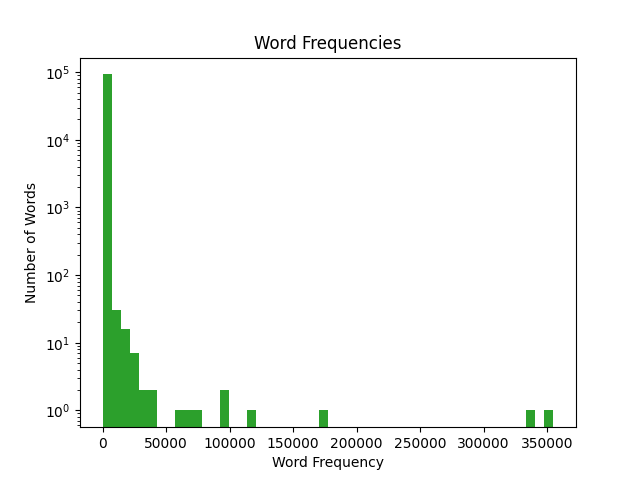
\includegraphics[width=0.5\textwidth]{"../data/word_frequencies.png"}
              \caption{Word Frequencies}
              \label{fig:my_label}
          \end{figure}

          In the Figure \ref{fig:my_label} you can see the distribution of the words.

          \textbf{Note:} My training loss and the validation loss is poor, but one of the ways I found to improve was through fixing the way I was removing the pairs from the original. I ended up using the itertools.chain function. I also increased the number of times the word should appear from 5 to 10. This really improved the way my training loss and validation loss decreased. However it still takes very long time to this filtering and would like to know if there is any other way to do this in the feedback.
    \item The final modified pairs were saved as a pkl file under \textbf{./data/}. This took a very long time to process and maybe my implementation could have definitely been better. I saw some other implementations online and tried to implement them but I did not got the results I wanted. If there is any way to improve this please let me know in the feedback.
    \item I have implemented a way in which it takes random sentences from the dataset. I used the \textbf{random.choice()} function to do this. For the standard training loop I took 20,000 sentences while for the loop with gradient accumulation I took 30,000 sentences.
    \item In this question we were asked to complete the class Vocabulary. What the purpose of this class is to build a Vocabulary from the list of sentence pairs (questions and answers) and then convert them to the words with the corresponding indices attached them. In the init method I intialize all the variables which are needed. Among those those variables the interesting one are word2index and index2word, which as the name suggests is a dictionary which maps the word to the index and vice versa. The other variable is the word2count which is a dictionary which maps the word to the number of times it occurs in the dataset.

          There are 3 methods in the class which are \textbf{add\_vocabularly}, \textbf{add\_sentence} and \textbf{add\_word}. The method \textbf{add\_vocabularly} iterates over all the sentences pairs and adds each sentence to the Vocabulary. It uses the function \textbf{add\_sentence} which basically breaks the sentnece into words and then finally uses the functions \textbf{add\_word} to add the word to the Vocabulary. The method \textbf{add\_word} adds the word to the Vocabulary and also updates the word2count dictionary.
\end{enumerate}

\section{Model \& Tools for training (35 pts)}
\begin{enumerate}
    \item The PositionalEncoding is a class which is used to add the positional encoding to the input. The positional encoding is added to the input so that the model can understand the position of the word in the sentence.

          The init constructor method is the method where the positional encoding for a given maximum length and dimension is calculated. It is then sorted in the buffer. It also uses the dropout parameter which is used to drop the input randomly. In the forward method the positional encoding is added to the input and then returned.

          This class is very commonly used in the Transformers models as it is very essential to make the model understand the position of the words in the sentence and their values.
    \item In this question we were asked to complete the init constructor method of the class TransformerModel. We were asked in total 4 tasks which were; Add an embedding layer, add a positional encoding layer, add a transformer layer. I will now explain what this constructor does a whole and how it is needed.

          The reason we add an embedding layer is because we need to convert the words into vectors. One of the parameters for it is the padding value, which is given so that it can ignore the padding tokens. Also the positional encoding layer is created through the PositionalEncoding class which I explained in the previous question. The Transformer layer is created because it is very important for the language processing as it is successful in performing well in these tasks. The reason why I have chosen to have batchfirst as true is because I wanted to specify the format of the input data. When the batchfirst is true then the input and output tensors are provided as (batch, seq, feature). This is the format which I wanted to have for my input and output tensors.
    \item This method called as createPaddingMask was rather simple in which I return a boolean which is either true or false if the token is equal to the padding token. This is done so that the model can ignore the padding tokens.
    \item In this question we were asked to complete the method forward. This method is used to pass the input through the model and then return the output. It takes in the source and target sequences and applies the entire sequence of operations which is defined in the Transformer Model. There are two types of masking applied here. The first type is the padding masks, which is used to ignore the padding tokens in the input data. The main use of padding is to make all the sentences of the same length. However when training the actual data we do not want it to be considered. The second type of masking is the Future Mask. This mask is used in the decoder part of the Transformer Model which is used to prevent each position from attending the future positions. This is done so that the model can not cheat and look at the future tokens and then predict the output.
    \item The reason why the Transformer model is using the masks value as True / False and not as 0 and - infinity because of the way PyTorch handles the masks. In PyTorch the masks are used as a boolean value and not as a number. In PyTorch the masks are expected to be boolean tensers, where True values correspond to positions that should be ignored. When the mask is applied, the positions with the True values are set to -infinity. after the attention scores are computed, the softmax function is applied and the -infinity values become zeros again. This is the reason why we use True / False and not 0 and -infinity.
\end{enumerate}

\section{Training (35 pts)}
\begin{enumerate}
    \item In this we are asked to implement the Standard Training Loop to make a model which can predict the response to inputs and act as a Chat Bot. The implementation wsa done in a very basic way. 

          I have decided to use (after many trial and errors with different optimizer) Adam optimizer. I have also used the learning rate scheduler which is using the StepLR class. The Loss function is the CrossEntropyLoss which again was chosen from multiple trial and errors with different loss functions. The important part of this (which I found later from updated project description) was to ignore the padded sequence in the loss function. This was very important because otherwise I was getting training loss and validation loss bellow 1.5 within 2 to 3 epochs. The training loop itself is also very straight forward. It iterated over the training data and then prepares the decoder input and target to perform the forward pass. It calculates the lass for each batch and calculates that. After each epoch it also calculates the learning rate again which is adjusted according to the scheduler. Also if the validation loss does not decrease for a certain number of epochs the function stops early (early stopping). The model is then saved as a pkl file under \textbf{./data/}.

          The hyperparameters which I have used are the same as the one provided in the Remarks. The number of epochs which is used is 20. Bellow you can see the graphs showing the training loss and validation loss.

          \begin{figure}[H]
              \centering
              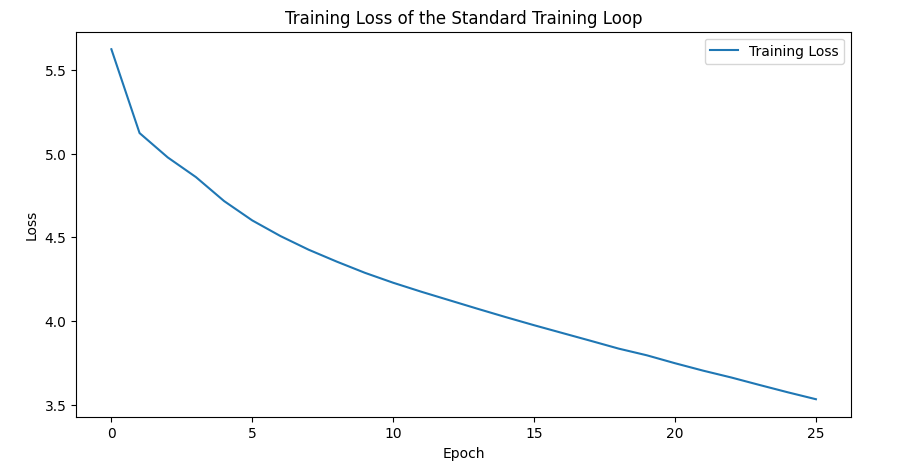
\includegraphics[width=0.5\textwidth]{"../data/training_loss_simple_training_loop.png"}
              \caption{Training Loss for Standard Training Loop}
              \label{fig:my_label}
          \end{figure}

          \begin{figure}[H]
              \centering
              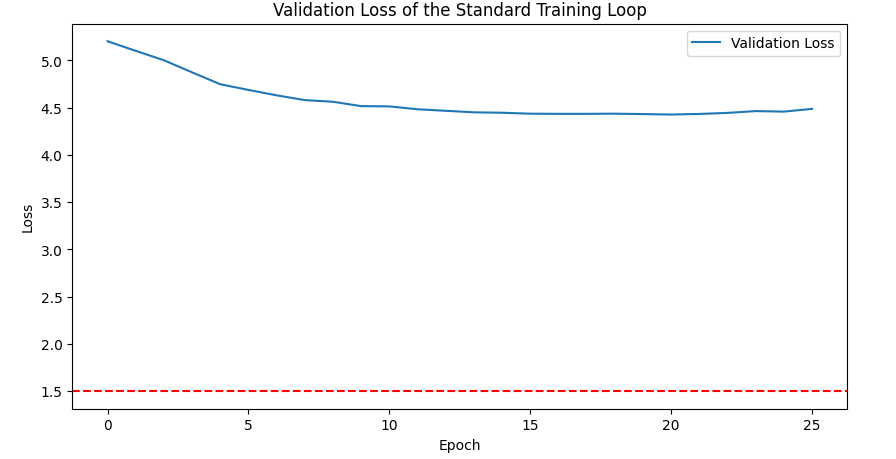
\includegraphics[width=0.5\textwidth]{"../data/validation_loss_simple_training_loop.png"}
              \caption{Validation Loss for Standard Training Loop}
              \label{fig:vmodel1}
          \end{figure}

          In the above Figure \ref{fig:my_label} and Figure \ref{fig:vmodel1} the training and validation loss can be seen. As it can be seen from above both the Validation Loss and the Training Loss are not good. I tried multiple ways to get better convergence but I did not get the results which I am satisfied with. I tried to change the optimizer, loss function adn the learning rate scheduler but they all lead to having a very unstable training and validation loss. This is the best results which I got from all of my combinations. I would like to also know what I could have done better to get better results in the feedback, as I took these extra days to try and improve the results but I could not get much better results.
    \item In this training loop we were asked to replace the standard loss computation and instead implement the Gradient accumulation. The reason why we use gradient accumulation is because it is very useful when we have limited GPU memory. As it can be seen in the code every some iterations we perform the backward pass and the update the parameters. Everything is else is the same as the standard training loop.

          The hyperparameter which I have used are the same as the one provided in the Remarks. The number of epochs which is used is 20 with early stopping implemented. Bellow you can see the Training and Validation Loss.

          \begin{figure}[H]
              \centering
              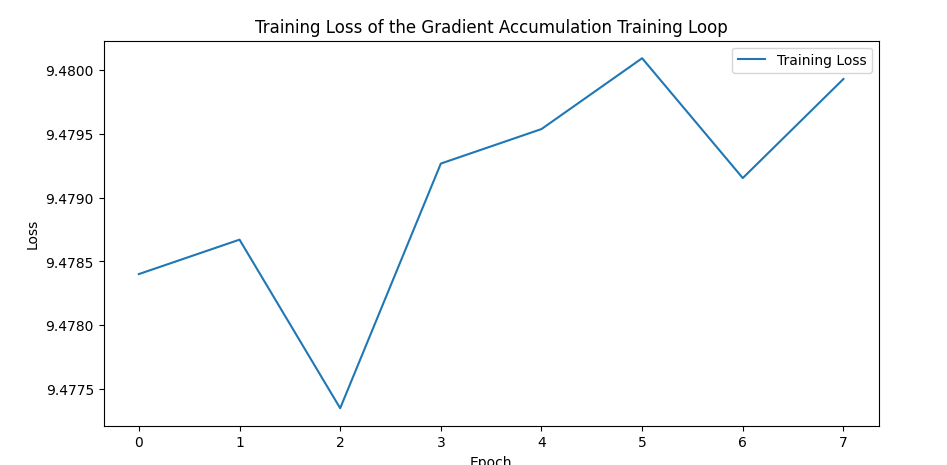
\includegraphics[width=0.5\textwidth]{"../data/training_loss_gradient_accumulation.png"}
              \caption{Training Loss for Gradient Accumulation}
              \label{fig:tmodel2}
          \end{figure}

          \begin{figure}[H]
              \centering
              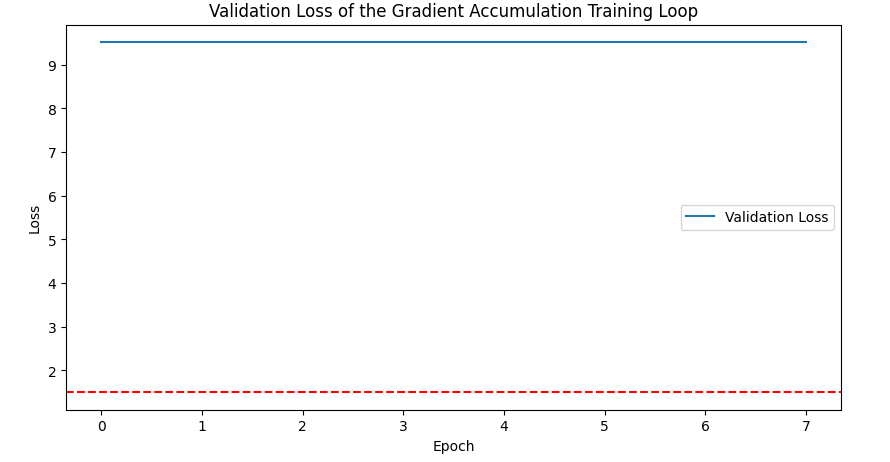
\includegraphics[width=0.5\textwidth]{"../data/validation_loss_gradient_accumulation.png"}
              \caption{Validation Loss for Gradient Accumulation}
              \label{fig:vmodel2}
          \end{figure}

          In the above Figure \ref{fig:tmodel2} and Figure \ref{fig:vmodel2} the training and validation loss can be seen. These results were even more disappointing for me as I expected which this implementation to get better results. The problem is that it does not even improve at all, it says at a constant learning and validation loss. I do believe that maybe in my implementation I have made some mistake, but even taking these extra days I could not figure out how to get the results which I wanted. I would like to know what I could have done better in the feedback as well for this.
\end{enumerate}

\section{Evaluation (10 pts)}
\begin{itemize}
    \item In this question we are asked to implement the greedy decoding in which we are supposed to select the word with the highest probability. The greedy decoding function is used in sequence-to-sequence models, particularly in Natural Language Processing (NLP). It generates an output sequence from a given input sequence using a trained transformer model. The function selects the word with the highest probability as the next word in the sequence. This selection is done using the torchargmax() function, which returns the index of the maximum value in a tensor. The function creates a target\_input tensor, which is filled with the start token, and then iteratively adds the most probable next word to the sequence until the end-of-sequence token is reached or the maximum sequence length is achieved.
    \item In this question we asked to implement the tok-k-sampling in which it takes the top 5 next words and choses a random words from them. The way I have done is by making a probability out of all the possible words and then taking the top 5 words for that. I then take a random work from those top 5 words and use that as the next sentence.
    \item In the bellow table I have shown the output of the both the models with Greedy Strategy and Top K Sampling Strategy. I have only taken the maximum sentence length as 5 words, because from my testing then only does the sentences make more sense.

          \begin{table}[H]
              \centering
              \begin{tabular}{|l|l|l|}
                  \hline
                  \multicolumn{3}{|c|}{Evaluating of the model: Standard Model}                                         \\
                  \hline
                  Method                           & Input                          & Output                            \\
                  \hline
                  \multirow{3}{*}{Greedy Decoding} & Where are you?                 & quiet welcome Hurry hop           \\
                                                   & how are you doing?             & checked Side yesterday, checked   \\
                                                   & I am doing great how about you & donít pint fund Irene             \\
                  \hline
                  \multirow{3}{*}{Top-K Decoding}  & Where are you?                 & bringing district Donald Seymour  \\
                                                   & how are you doing?             & babbling keys theory, Honey       \\
                                                   & I am doing great how about you & Loomis like, demonstration scream \\
                  \hline
              \end{tabular}
              \caption{Model Evaluation Results for Standard Model}
              \label{tab:standard_model_results}
          \end{table}

          The table \ref{tab:standard_model_results} shows the results for the Standard Model. As it can be seen the results are not very good. The sentences do not make much sense and are very random. The reason for this is because the model is not trained well and hence it is not able to predict the next word properly. However if we now compare the Greedy Decoding and Top-K Decoding it can be seen that both do not really make much difference. To an extend I do feel it is trying to make some sense, but it has not learned properly how to formulate sentences.

          \begin{table}[H]
              \centering
              \begin{tabular}{|l|l|l|}
                  \hline
                  \multicolumn{3}{|c|}{Evaluating of the model: Gradient Accumulation Model}                            \\
                  \hline
                  Method                           & Input                          & Output                            \\
                  \hline
                  \multirow{3}{*}{Greedy Decoding} & Where are you?                 & end, cool hid Cops                \\
                                                   & how are you doing?             & director stand, me, Continue      \\
                                                   & I am doing great how about you & woulda Sick photo brandy          \\
                  \hline
                  \multirow{3}{*}{Top-K Decoding}  & Where are you?                 & engineer Tommy Chicken bed,       \\
                                                   & how are you doing?             & Where're minute, B executive      \\
                                                   & I am doing great how about you & like restraining Hopefully Viktor \\
                  \hline
              \end{tabular}
              \caption{Model Evaluation Results for Gradient Accumulation Model}
              \label{tab:my_label}
          \end{table}


          The table \ref{tab:my_label} shows the results for the Gradient Accumulation Model. The results above are more disappointing than the Standard Model. The reason for this is because the model trained worse as compare to the standard model.
    \item Overall I am not satisfied with this project as I am not sure how I could have improved the model more. I took the extra days as well in hope of getting a better trained model, but I feel that it was not worth it. I tried also the suggestions which were given during the lectures. For instance I tried implementing the Xavier Normalization as well, but that just made the learning rate and validation rate very inconsistent. I tried adding other layers as well (suggested mainly from ChatGPT) but they also gave very inconsistent results. I do hope that in the feedback I can get some suggestions on how I could have improved the model more because later on I would love to work on this project more and make it better. Maybe in hindsight I should have taken this extra time to finish the bonus.

\end{itemize}






\end{document}
